\documentclass{article}
\usepackage{amsmath,amssymb}
\usepackage{tikz}
\usepackage{pgfplots}
\pgfplotsset{compat=1.18}
\begin{document}
\section{Example}
Text and integers 12345; decimal 3.14159; Vietnamese Unicode: Toán học.
Inline math: $x^2+2x+1=(x+1)^2$.
\begin{equation}
\int_0^1 x^2\,dx=\frac{1}{3}.
\end{equation}
\begin{figure}[ht]
\centering
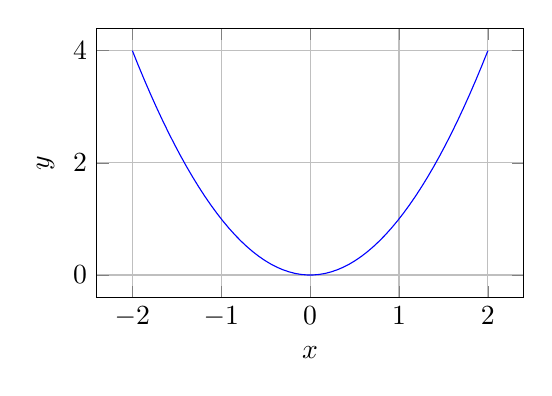
\begin{tikzpicture}
  \begin{axis}[width=7cm,height=5cm,xlabel={$x$},ylabel={$y$},grid=major]
    \addplot[blue,domain=-2:2,samples=60]{x^2};
  \end{axis}
\end{tikzpicture}
\caption{Illustrative plot generated with PGFPlots.}
\end{figure}
\begin{tabular}{|l|r|}
\hline Item & Value \\ \hline A & 25 \\ B & 35 \\ \hline
\end{tabular}
\end{document}
